\documentclass[11pt,spanish]{article}
\usepackage[spanish]{babel}
\selectlanguage{spanish}
\usepackage[utf8]{inputenc}
\usepackage{graphicx}
\usepackage{caption}
\usepackage{subcaption}
\usepackage{hyperref}

\begin{document}

\title{Redes Neuronales Profundas: Trabajo Práctico 2}
\date{}
\maketitle

\section*{Respuestas}
El código realizado para la resolución de los ejercicios está disponible en \href{https://github.com/dncampo/deep-learning/tree/lpineda}{github} (branch \textit{lpineda})

\subsection*{Ejercicio 1}
El ejercicio tutorial propuesto consiste en definir una función $f(x,y) = x^2+2xy+y^2$ en Theano. La única modificación debe realizarse en la variable ``out''. \par

Para el ejemplo de regresion lineal, se separa el dataset en mini-batches para ir entrenando el modelo de forma progresiva, utilizando subconjuntos de datos. 
Con el dataset de motos y aviones de Caltech101, las imagenes son leidas y apiladas como vectores en una matriz que representa el dataset, y cada clase se representa con un vector de 0 o un 1. Luego el entrenamiento se realiza por épocas, finalizando cuando el error de entrenamiento no varia más que cierto umbral en las últimas 50 épocas o por máximo de iteraciones. La evolución del error de entrenamiento y test se puede observar en la figura \ref{ex1b2}
\begin{figure}[htbp]
	\centering
	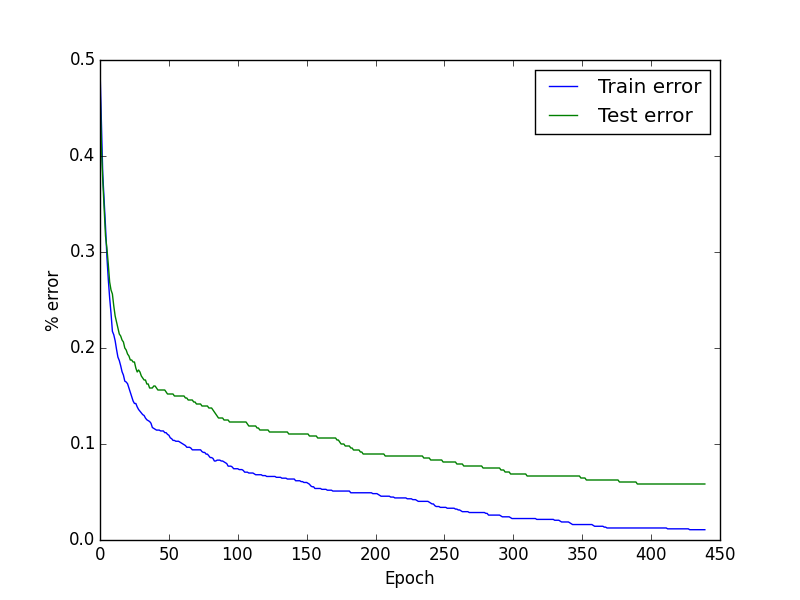
\includegraphics[width=0.5\textwidth]{../ex1b2.png}
	\caption{Error de train y test}
	\label{ex1b2}
\end{figure}

Finalmente, para la tercera parte de este ejercicio se debe agregar al model una capa oculta de 100 neuronas con activación ReLU. Para esto es necesario definir una nueva matriz de pesos y un nuevo vector de bias para esta capa oculta. Además, se debe modificar la función de actualización para que calcule los delta usando los gradientes de la capa oculta. El entrenamiento se realiza de la misma manera que en el ejemplo de regresión lineal. La evolución del error de entrenamiento y test se puede observar en la figura \ref{ex1b3}

\begin{figure}[htbp]
	\centering
	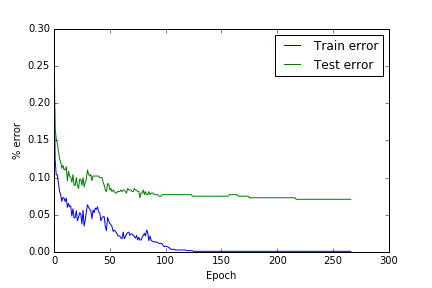
\includegraphics[width=0.5\textwidth]{../ex1b3.png}
	\caption{Error de train y test de modelo con capa oculta de 100 neuronas}
	\label{ex1b3}
\end{figure}
\subsection*{Ejercicio 2}

\end{document}
